%\documentclass[aps,prl,twocolumn,showpacs,superscriptaddress,groupedaddress]{revtex4}
%% for review and submission
%\documentclass[aps,preprint,showpacs,superscriptaddress,groupedaddress]{revtex4}
% for double-spaced preprint
%\documentclass[aps,prl,floatfix,twocolumn,10pt]{revtex4-1}
%for review and submission
\documentclass[english]{nature} 
% for double-spaced preprint
%\documentclass[aip,apl,amsmath,amssymb,floatfix,preprint,a4paper]{revtex4-1}
%\documentclass[aip,apl,amsmath,amssymb,floatfix,reprint,a4paper]{revtex4-1}

%% Packages
\usepackage[T1]{fontenc}
\usepackage[utf8]{inputenc} %Umlaute
\usepackage{babel}
\usepackage{acronym}
\usepackage{amsmath}
\usepackage{amssymb}
\usepackage[bf,small,labelsep=period]{caption}
\usepackage{graphicx}  %figures
\usepackage[detect-all]{siunitx}
\usepackage[affil-it]{authblk}

%% New commands
\newcommand{\msub}[1]{\ensuremath{\textnormal{\begin{tiny}#1\end{tiny}}}}
\renewcommand{\d}[1]{\ensuremath{\operatorname{d}\!{#1}}}
\DeclareSIUnit{\voltpeak}{Vp}

%acronyms
\acrodef{CT}{computed tomography}
\acrodef{SNR}{signal-to-noise ratio}
\acrodef{CNR}{contrast-to-noise ratio}
\acrodef{SEM}{scanning electron microscope}
%% ----------------------------------------------------------------------------------------------------------------

\begin{document}

\title{X-ray phase-contrast imaging at \SI{100}{\kilo\electronvolt} on
a conventional source}

\author[1,2]{T.~Thüring}
\author[1,2]{M.~Abis}
\author[1]{Z.~Wang}
\author[1]{C.~David}
\author[1,2]{M.~Stampanoni}
\affil[1]{Paul Scherrer Institute, Villigen PSI, Switzerland}
\affil[2]{Institute for Biomedical Engineering, Swiss Federal Institute of Technology, Zurich, Switzerland}

\date{\today}


\maketitle

%%%%%%%%%%%%%%%%%%%%%%%%%%%%%%%%%%%%%%%%%%%%%%%%%%%%%%%%%%%%%%%%%%%%%%%%
% Body of manuscript
%%%%%%%%%%%%%%%%%%%%%%%%%%%%%%%%%%%%%%%%%%%%%%%%%%%%%%%%%%%%%%%%%%%%%%%%

%% ----------------------------------------------------------------------------------------------------------------
\begin{abstract}
    X-ray grating interferometry is a promising imaging technique sensitive
    to attenuation, refraction and scattering of the radiation. Applications
    of this technique in the energy range between $\num{80}$ and
    $\SI{150}{\kilo\electronvolt}$ pose severe technical challenges, and are
    still mostly unexplored. Phase-contrast X-ray imaging at such high
    energies is of relevant scientific and industrial interest, in
    particular for the investigation of strongly absorbing or thick materials 
    as well as for medical imaging. Here we show the successful
    implementation of a Talbot-Lau interferometer operated at
    $\SI{100}{\kilo\electronvolt}$ using a conventional X-ray tube and a
    compact geometry, with a total length of $\SI{54}{\centi\metre}$. We
    present the edge-on illumination of the gratings in order to overcome
    the current fabrication limits. Finally, the curved structures match
    the beam divergence and allow a large field of view on a short and
    efficient setup.
\end{abstract}

X-ray radiography and \ac{CT} are standard imaging techniques in
materials and life sciences for the nondestructive examination of samples or
diagnostic tasks in medicine. The underlying contrast mechanism
relies on the different X-ray attenuation properties of different materials
or tissue types. The dominant physical effects contributing to attenuation
are the photoelectric effect and incoherent (Compton) scattering. Besides attenuation, the wave
nature of X-rays reveals another contrast mechanism, which is the phase
shift. The interaction contributing to phase shifts is coherent (Rayleigh)
scattering~\cite{Als-Nielsen2011}.

The attenuation and phase shift properties are described by the complex
refractive index $n=1 - \delta + i \beta$. The imaginary part $\beta$ is
related to the attenuation coefficient by $\mu = 4 \pi \beta(\lambda) /
\lambda$, while the real part $\delta(\lambda)$ determines the phase shift
$\phi = 2 \pi \delta(\lambda) / \lambda$.

While the attenuation can be measured with an X-ray detector as the
reduction of the beam intensity, the phase is not directly observable.
Therefore, an optical system is needed to convert the phase shift into
intensity modulations.

Phase-sensitive imaging is a desirable modality, since it delivers a
complementary source of contrast with respect to absorption by providing
direct access to the electron density~\cite{Als-Nielsen2011}. Moreover, the
combination with attenuation enables the determination of the effective
atomic number~\cite{Qi2010}. An enhanced \ac{CNR} compared to
attenuation for certain materials or
tissues~\cite{Pfeiffer2007a,McDonald2009} has also been demonstrated.

The vast majority of phase-sensitive techniques, including crystal analyzer
based~\cite{Davis1995,Chapman1997} or
interferometric~\cite{Bonse1965,Momose1996} methods rely on X-ray beams of
high spatial and temporal coherence, which are available only at synchrotron
sources. Inline phase contrast~\cite{Snigirev1995,Wilkins1996,Cloetens1996}
and Talbot interferometry~\cite{Cloetens1997,David2002,Momose2003a} need
high spatial coherence but are available on polychromatic microfocus
sources. Phase-contrast imaging using X-ray beams of low temporal \emph{and}
spatial coherence such as conventional low-brilliance X-ray tubes have been
demonstrated with coded apertures~\cite{Munro2012} and Talbot-Lau
interferometry~\cite{Pfeiffer2006}. Analyzer-based systems have been
recently extended to tube sources~\cite{Nesch2009,Parham2009} but only at
energies up to the tungsten $K_\alpha$ line at~\SI{60}{\kilo\eV}. In
addition to phase sensitivity, crystal analyzers and Talbot interferometers
also provide --- with different retrieval mechanisms --- information
about the integrated local small angle scattering power from microscopic
density fluctuations in a specimen~\cite{Pfeiffer2008}. This signal is known
under the name of dark-field, scatter or visibility reduction contrast.

High-energy Talbot interferometry has been reported so far using a
synchrotron source at nominal energies of
$\SI{82}{\kilo\electronvolt}$~\cite{Willner2013}. Using a low-brilliance
X-ray tube, Talbot-Lau interferometry was applied so far at
$\SI{60}{\kilo\electronvolt}$ mean energy~\cite{Donath2009}. Medical imaging
applications may benefit from phase contrast at higher energies: chest or
abdominal radiography or \ac{CT} require an acceleration voltage between
\num{100} and $\SI{150}{\kilo\voltpeak}$. Other potential applications are
homeland security or chip failure analysis, which require high energies for
the visualization of materials of high density and atomic number.

\section*{Results}
We introduce a method for phase contrast imaging which works on
conventional X-ray sources, covers the entire diagnostic X-ray energy range
and is compatible with compact imaging arrangements. The approach is based
on Talbot-Lau interferometry~\cite{Pfeiffer2006} and employs an edge-on
illumination approach for the grating design and arrangement. Our solution
removes one of the major hurdles which prevented grating interferometry from
being
applied at high energies so far, namely the fabrication of
gratings with high aspect ratios. The aspect ratio, given by
\begin{equation}
    \text{R} = \frac{2h}{p},
\end{equation}
where $p$ is the
grating period and $h$ the  structure height, is limited by the
fabrication process, usually photolithography~\cite{David2002} or X-ray
lithography~\cite{Mohr2012} since grating structures tend to collapse or deform
(e.g.\ due to capillary forces) if the aspect ratio is too high. For a given
setup length these parameters depend on the target energy $E$ according to
$p \propto 1/\sqrt{E}$ and $h \propto E^3$, and therefore $\textnormal{R}
\propto E^{7/2}$~\cite{Momose2003a}. If at $E=\SI{25}{\kilo\electronvolt}$
an aspect ratio for the absorption grating around $\textnormal{R}=30$ is
sufficient, it would
have to be at least $128$ for $E=\SI{100}{\kilo\electronvolt}$. Moreover,
when using a broad spectrum, photons above the design energy should also be
efficiently blocked by the gratings, thus requiring even higher aspect
ratios. The largest aspect ratios achieved by current fabrication
techniques~\cite{David2007,Kenntner2010} are around 60.

Our design introduces edge-on illuminated,  circularly aligned structures. Edge-on illumination
(Fig.~\ref{Fig:schematic}), as
opposed to face-on illumination, exploits the dimension along the grating
lines to form a high aspect ratio of the structures in the direction of the beam. The
effective structure height of the grating is then determined by the grating
dimension along the grating lines, which essentially allows arbitrarily high
aspect ratios. 
\begin{figure}[h!]
    \centering
    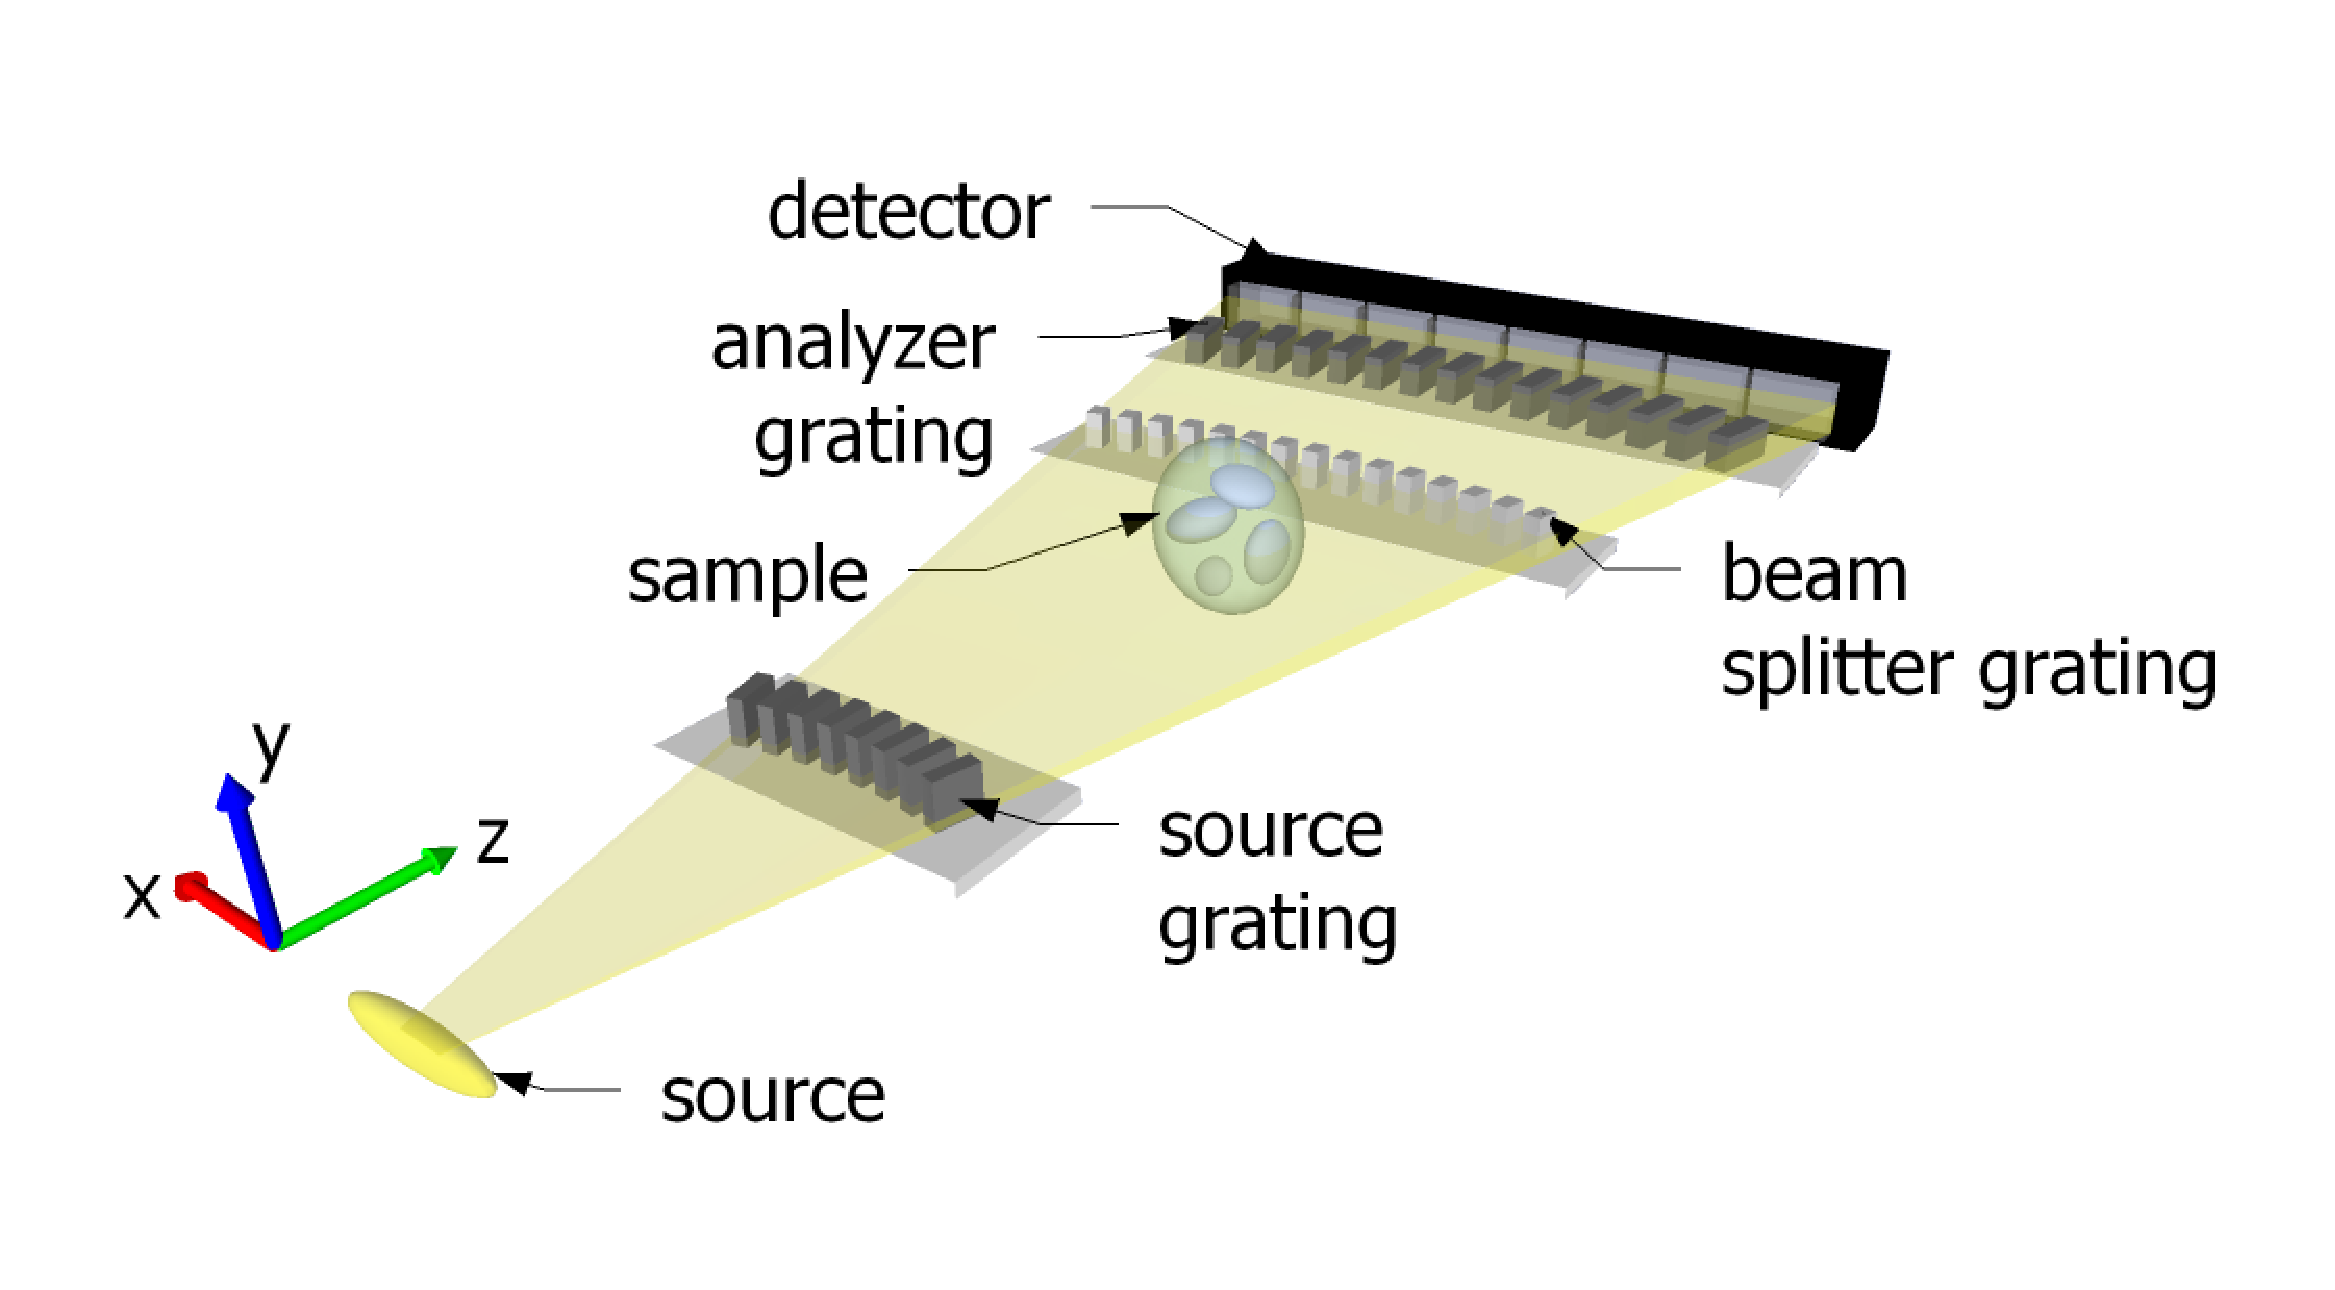
\includegraphics[width=.7\textwidth]{figures/figure1.eps}
    \caption{Schematic of a grating
        interferometer for X-ray energies between 60 and
        \SI{150}{\kilo\electronvolt} in edge-on illumination mode. The
        aspect ratio is defined by the ratio of the travelling distance along the
        grating lines and the period and can be arbitrarily long. In order to maximise
        the field of view, the grating structures are aligned on an
        arc. A \SI{100}{\kilo\eV} setup was realised where the distance
        between the source and the source grating is \SI{23}{\centi\metre}
    and the distance between the source grating and the phase grating is
    \SI{16}{\centi\metre}. That is also the distance from the phase grating
to the analyzer grating.}%
\label{Fig:schematic}
\end{figure}

Increasing the aspect ratio of the gratings typically leads to a
reduction of the field of view due to the change of the grating transmission
function at high incident angles. In order to overcome this problem, the grating lines are circularly aligned 
with a radius equal to the distance to the source. 
This allows to achieve an arbitrarily large field of view in a fan-beam
geometry, a significant improvement compared to face-on based and glancing
angle~\cite{Stutman2012a} approaches.

The combination of edge-on illumination and circularly aligned structures
enables phase-contrast imaging at arbitrary design energies and with a
maximum field of view in the horizontal direction ($x$ direction). These
advantages come at the expense of a limited field of view in the vertical
direction ($y$ direction), which is, depending on the X-ray detector,
typically a few pixels. 
However, radiographic 2D imaging can be obtained by scanning the sample or a thin fan
beam. The scanning technique has been demonstrated to deliver less dose than
the conventional approach based on the illumination of a large area. In
digital mammography, for instance, where dose is a critical issue, Philips'
MicroDose system combines a scanning approach with an highly collimated fan
beam~\cite{Aslund2007}. Thanks to the high collimation, the dose deposited
on  patients has been reported to be significantly lower than with other
instruments based on the illumination of a large area
detector~\cite{Oduko2010}.
Similarly, for tomographic images,
the approach allows single slice \ac{CT} or full 3D imaging in scanning mode.

Grating design and fabrication is nonstandard and involves a complex mask
design, as shown in Fig.~\ref{Fig:grating_mask}. Multiple gratings can reside on a
silicon chip with their specific structure length and curvature. For the
current experiments, a symmetric interferometer with a grating period of $p
= \SI{2.8}{\micro\metre}$ for all gratings has been used. The design energy
is $\SI{100}{\kilo\electronvolt}$ and the beam splitter grating periodically
shifts the phase by zero and $\pi$ at this energy~\cite{David2002}. Using
gold as the phase shifting material, a structure length of
$h_1 = \SI{19.8}{\micro \metre}$ is required. The analyzer grating is an absorption mask
for sensing slight changes of the interference pattern generated by the beam
splitter~\cite{Momose2003a}. With a structure length of $h_2 =
\SI{800}{\micro \metre}$
it can absorb more than \SI{70}{\percent} of the incoming X-rays up to energies of 
$\SI{160}{\kilo\electronvolt}$. The beam splitter and analyzer grating are
separated at the first fractional Talbot order~\cite{Weitkamp2005},
resulting in an intergrating distance of $\SI{158}{\milli\metre}$. The
source grating splits the relatively large focal spot ($\sim
\SI{1}{\milli\metre}$) into an array of individually coherent, but mutually
incoherent sources~\cite{Pfeiffer2006}. It is also made of gold structures
with a length of $h_0 = h_2 = \SI{800}{\micro \metre}$.
\begin{figure}[h!]
    \centering
    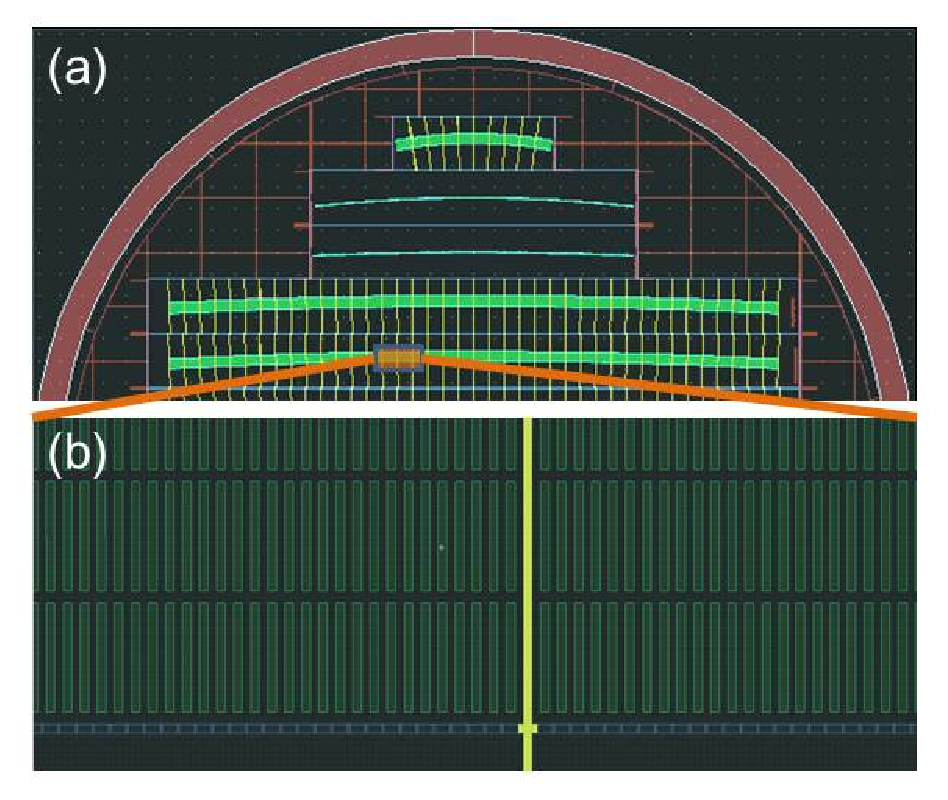
\includegraphics[width=.6\textwidth]{figures/grating_mask.eps}
    \caption{Grating design mask for
        the edge-on illumination approach and \ac{SEM}
        image of the grating. The top part of the 4 inch wafer shows
        five grating chips. From top to bottom, one source grating, two
        phase gratings and two analyzer gratings. The
        gratings have different curvatures which are specific to the grating
        interferometer geometry. 
        The \ac{SEM} image shows the gold structures and the interrupting bridges
        that prevent the lamellae from collapsing~\cite{Kenntner2010}.}\label{Fig:grating_mask}
\end{figure}

Due to the large spectral acceptance~\cite{Weitkamp2005,Thuering2013c} of the
interferometer ($\SI{50}{\kilo\electronvolt}$ to
more than $\SI{160}{\kilo\electronvolt}$) and the high attenuation efficiencies of
the source and analyzer gratings ($>90\%$ up to
$\SI{160}{\kilo\electronvolt}$), the voltage of the X-ray source was set to
the maximum of $\SI{160}{\kilo\volt}$. With a structure height of
approximately $\SI{100}{\micro \metre}$, the field of view in the vertical
direction is limited to one detector pixel row. In the horizontal direction,
the field of view is only limited by the grating size to
$\SI{30}{\milli\metre}$, but wider gratings can be fabricated with the same
method and the available technology on larger wafers. In addition to the standard components (source,
camera, interferometer), two optical slits, one in front of the source
grating, the other in front of the camera, were required for the collimation
of the beam in the vertical direction. 

\section*{Discussion}
Several resistors and an integrated circuit are located on different layers
on the electronic chip in fig.~\ref{Fig:img_chip}. The radiographs were
acquired in scanning mode, using a step size of
$\SI{100}{\micro \metre}$ along the $y$ axis. For a better comparison of the
magnified phase and attenuation images, the attenuation image has been
replaced with the differential attenuation image, which was obtained by
calculating the derivative along the horizontal axis. In the attenuation
image, the contrast of the soldering points of
the integrated circuit is reduced underneath the resistors, while in
the phase image, they can clearly be identified. The reduced contrast of the 
soldering points in the absorption image is due to beam hardening. The spectrum
impinging on these soldering point is hardened by the resistors in the upper
layer, resulting in lower absorption contrast. Due to the weaker energy
dependence of phase shifts ($1/E$ compared to $1/E^3$), phase-contrast images
are less sensitive to beam hardening~\cite{Chabior2011a}, which explains the
lower contrast reduction of the soldering points underneath the resistors in the
phase image of the chip. This result shows the benefit of the phase contrast in
high-energy X-ray imaging, which may be useful to identify flaws in multilayered
structures such as electronic chips.
\begin{figure}[h!]
    \centering
    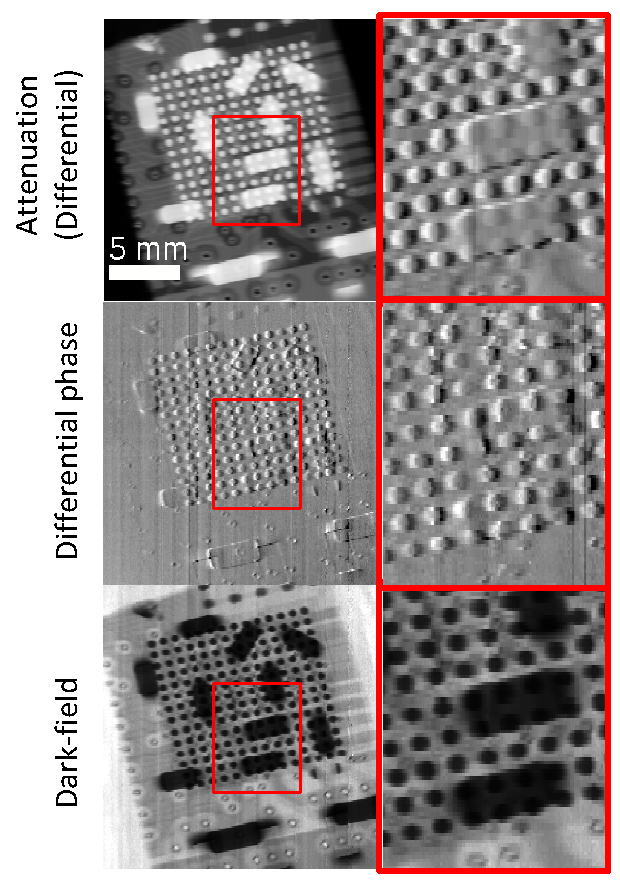
\includegraphics[width=.5\textwidth]{figures/img_chip_dabs.eps}
    \caption{Radiographic scan of an electronic chip. The image was acquired
        with 24 phase steps per line and an exposure time of \SI{15}{\second} per
    step. The top right image shows the differential absorption image.}\label{Fig:img_chip}
\end{figure}

Edge-on illuminated grating interferometry finally allows phase contrast
imaging to be performed at high energies ($>\SI{100}{\kilo\eV}$) on conventional X-ray
sources. With a circular alignment of the gratings, the diffracting and
absorbing structures can be matched to the divergent beam, even for very
compact geometries. Short, high-energy phase-contrast systems enable the
efficient investigation of high-density materials or thick samples,
adding information on electron density and integrated small angle scattering
power to the conventional absorption based signal. This will improve
material discrimination and density sensitivity capabilities in future
X-rays or even neutron~\cite{Grunzweig2008} investigations.

\section*{Methods}
Edge-on illuminated gratings were manufactured by Microworks GmbH, Germany, using a LIGA process~\cite{Kenntner2010}. Each grating
resides on a $5 \times \SI{60}{\milli\metre^2}$ silicon chip and several
grating chips are fabricated on a single 4 inch silicon wafer. The
experimental arrangement for a design energy at \SI{100}{\kilo\electronvolt}
is a symmetric Talbot-Lau interferometer with a grating period of $p =
\SI{2.8}{\micro \metre}$ for all gratings. The distance from the source
grating to the analyzer grating is $\SI{32}{\centi\metre}$ and the source
grating is positioned $\SI{23}{\centi\metre}$ away from the source.

The X-ray source is a COMET MXR-160HP/11 X-ray tube with a maximum output
voltage of $\SI{160}{\kilo\volt}$. In the experiment, it was set to the
maximum voltage. The focal spot size is approximately
$\SI{1}{\milli\metre}$. The detector is a CCD camera from Finger Lakes
Instruments. A cesium iodide (CsI:Tl) scintillator of $\SI{600}{\micro
\metre}$ thickness converts the X-rays to visible light and is coupled to
an optical lens projecting the image onto the CCD\@. The effective pixel size
is $\SI{80}{\micro\metre}$. The collimating slit right after the source is 
$\SI{25}{\micro\metre}$ wide, while the second slit before the detector is
$\SI{100}{\micro\metre}$.

In Fig.~\ref{Fig:img_chip}, image acquisition involved 24 phase steps per
line and an exposure time of 15 seconds per step. The long
exposure times are mostly constrained by the low average visibility of the
gratings (\SI{5}{\percent}). The exposure time was chosen in order to
get a low noise in the differential phase image. The \ac{SNR} is
proportional to the visibility and the square root of the exposure
time~\cite{Raupach2011}.
This implies that the exposure times can easily drop by an order of
magnitude as these gratings become comparable in quality to those developed
in the last ten years. 
Smaller regions of these gratings already exhibit a visibility up
to~\SI{14}{\percent}, indicating that this goal is reachable as the
fabrication becomes more reliable and uniform.

\section*{Acknowledgements}
We thank Gordan Mikuljan, Peter Modregger and István Mohácsi from the Paul
Scherrer Institute (PSI), Switzerland, for the
work on the mechanical design, the scientific advice, and the \ac{SEM} images
respectively, Joachim Schulz and Marco Walter from
Microworks GmbH, Germany, for the competent support on grating design
issues, Christian Kottler and Vincent Revol from Centre Suisse
d'Electronique et de Microtechnique (CSEM), Switzerland for the fruitful
discussions on the design of the system. This work has been partially
supported by the Competence Centre for Materials Science and Technology
(CCMX) of the ETH Board, Project Nr. 61 and by the ERC Grant ERC-2012-StG 310005-PhaseX.

\section*{Additional information}
The authors declare no competing financial interests.

%\bibliographystyle{naturemag-nourl}
%\bibliography{library}
\begin{thebibliography}{10}
\expandafter\ifx\csname url\endcsname\relax
  \def\url#1{\texttt{#1}}\fi
\expandafter\ifx\csname urlprefix\endcsname\relax\def\urlprefix{URL }\fi
\providecommand{\bibinfo}[2]{#2}
\providecommand{\eprint}[2][]{\url{#2}}

\bibitem{Als-Nielsen2011}
\bibinfo{author}{Als-Nielsen, J.} \& \bibinfo{author}{McMorrow, D.}
\newblock \emph{\bibinfo{title}{{Elements of modern X-ray physics}}}
  (\bibinfo{year}{2011}).

\bibitem{Qi2010}
\bibinfo{author}{Qi, Z.}, \bibinfo{author}{Zambelli, J.},
  \bibinfo{author}{Bevins, N.} \& \bibinfo{author}{Chen, G.-H.}
\newblock \bibinfo{title}{{Quantitative imaging of electron density and
  effective atomic number using phase contrast CT.}}
\newblock \emph{\bibinfo{journal}{Physics in medicine and biology}}
  \textbf{\bibinfo{volume}{55}}, \bibinfo{pages}{2669--77}
  (\bibinfo{year}{2010}).

\bibitem{Pfeiffer2007a}
\bibinfo{author}{Pfeiffer, F.} \emph{et~al.}
\newblock \bibinfo{title}{{High-resolution brain tumor visualization using
  three-dimensional x-ray phase contrast tomography.}}
\newblock \emph{\bibinfo{journal}{Physics in medicine and biology}}
  \textbf{\bibinfo{volume}{52}}, \bibinfo{pages}{6923--6930}
  (\bibinfo{year}{2007}).

\bibitem{McDonald2009}
\bibinfo{author}{McDonald, S.~A.} \emph{et~al.}
\newblock \bibinfo{title}{{Advanced phase-contrast imaging using a grating
  interferometer}}.
\newblock \emph{\bibinfo{journal}{Journal of Synchrotron Radiation}}
  \textbf{\bibinfo{volume}{16}}, \bibinfo{pages}{562--572}
  (\bibinfo{year}{2009}).

\bibitem{Davis1995}
\bibinfo{author}{Davis, T.}, \bibinfo{author}{Gao, D.},
  \bibinfo{author}{Gureyev, T.}, \bibinfo{author}{Stevenson, A.} \&
  \bibinfo{author}{Wilkins, S.}
\newblock \bibinfo{title}{{Phase-contrast imaging of weakly absorbing materials
  using hard X-rays}}.
\newblock \emph{\bibinfo{journal}{Nature}} \textbf{\bibinfo{volume}{373}},
  \bibinfo{pages}{595--598} (\bibinfo{year}{1995}).

\bibitem{Chapman1997}
\bibinfo{author}{Chapman, D.} \emph{et~al.}
\newblock \bibinfo{title}{{Diffraction enhanced x-ray imaging}}.
\newblock \emph{\bibinfo{journal}{Physics in Medicine and Biology}}
  \textbf{\bibinfo{volume}{42}}, \bibinfo{pages}{2015--2025}
  (\bibinfo{year}{1997}).

\bibitem{Bonse1965}
\bibinfo{author}{Bonse, U.} \& \bibinfo{author}{Hart, M.}
\newblock \bibinfo{title}{{An x-ray interferometer}}.
\newblock \emph{\bibinfo{journal}{Applied Physics Letters}}
  \textbf{\bibinfo{volume}{6}}, \bibinfo{pages}{155--156}
  (\bibinfo{year}{1965}).

\bibitem{Momose1996}
\bibinfo{author}{Momose, A.}, \bibinfo{author}{Takeda, T.},
  \bibinfo{author}{Itai, Y.} \& \bibinfo{author}{Hirano, K.}
\newblock \bibinfo{title}{{Phase-contrast X-ray computed tomography for
  observing biological soft tissues}}.
\newblock \emph{\bibinfo{journal}{Nature Medicine}}
  \textbf{\bibinfo{volume}{2}}, \bibinfo{pages}{473--475}
  (\bibinfo{year}{1996}).

\bibitem{Snigirev1995}
\bibinfo{author}{Snigirev, A.}, \bibinfo{author}{Snigireva, I.},
  \bibinfo{author}{Kohn, V.}, \bibinfo{author}{Kuznetsov, S.} \&
  \bibinfo{author}{Schelokov, I.}
\newblock \bibinfo{title}{{On the possibilities of x-ray phase contrast
  microimaging by coherent high-energy synchrotron radiation}}.
\newblock \emph{\bibinfo{journal}{Review of Scientific Instruments}}
  \textbf{\bibinfo{volume}{66}}, \bibinfo{pages}{5486--5492}
  (\bibinfo{year}{1995}).

\bibitem{Wilkins1996}
\bibinfo{author}{Wilkins, S.}, \bibinfo{author}{Gureyev, T.},
  \bibinfo{author}{Gao, D.}, \bibinfo{author}{Pogany, A.} \&
  \bibinfo{author}{Stevenson, A.}
\newblock \bibinfo{title}{{Phase-contrast imaging using polychromatic hard
  X-rays}}.
\newblock \emph{\bibinfo{journal}{Nature}} \textbf{\bibinfo{volume}{384}},
  \bibinfo{pages}{335--338} (\bibinfo{year}{1996}).

\bibitem{Cloetens1996}
\bibinfo{author}{Cloetens, P.}, \bibinfo{author}{Barrett, R.},
  \bibinfo{author}{Baruchel, J.}, \bibinfo{author}{Guigay, J.} \&
  \bibinfo{author}{Schlenker, M.}
\newblock \bibinfo{title}{{Phase objects in synchrotron radiation hard x-ray
  imaging}}.
\newblock \emph{\bibinfo{journal}{Journal of Physics D: Applied Physics}}
  \textbf{\bibinfo{volume}{29}}, \bibinfo{pages}{133--146}
  (\bibinfo{year}{1996}).

\bibitem{Cloetens1997}
\bibinfo{author}{Cloetens, P.}, \bibinfo{author}{Guigay, J.},
  \bibinfo{author}{{De Martino}, C.}, \bibinfo{author}{Baruchel, J.} \&
  \bibinfo{author}{Schlenker, M.}
\newblock \bibinfo{title}{{Fractional Talbot imaging of phase gratings with
  hard x rays.}}
\newblock \emph{\bibinfo{journal}{Optics letters}}
  \textbf{\bibinfo{volume}{22}}, \bibinfo{pages}{1059--61}
  (\bibinfo{year}{1997}).

\bibitem{David2002}
\bibinfo{author}{David, C.}, \bibinfo{author}{N\"{o}hammer, B.},
  \bibinfo{author}{Solak, H.} \& \bibinfo{author}{Ziegler, E.}
\newblock \bibinfo{title}{{Differential x-ray phase contrast imaging using a
  shearing interferometer}}.
\newblock \emph{\bibinfo{journal}{Applied Physics Letters}}
  \textbf{\bibinfo{volume}{81}}, \bibinfo{pages}{3287--3289}
  (\bibinfo{year}{2002}).

\bibitem{Momose2003a}
\bibinfo{author}{Momose, A.} \emph{et~al.}
\newblock \bibinfo{title}{{Demonstration of X-Ray Talbot Interferometry}}.
\newblock \emph{\bibinfo{journal}{Japanese Journal of Applied Physics}}
  \textbf{\bibinfo{volume}{42}}, \bibinfo{pages}{L866--L868}
  (\bibinfo{year}{2003}).

\bibitem{Munro2012}
\bibinfo{author}{Munro, P.}, \bibinfo{author}{Ignatyev, K.},
  \bibinfo{author}{Speller, R.} \& \bibinfo{author}{Olivo, A.}
\newblock \bibinfo{title}{{Phase and absorption retrieval using incoherent
  X-ray sources}}.
\newblock \emph{\bibinfo{journal}{Proceedings of the National Academy of
  Sciences}} \textbf{\bibinfo{volume}{2012}}, \bibinfo{pages}{2--7}
  (\bibinfo{year}{2012}).

\bibitem{Pfeiffer2006}
\bibinfo{author}{Pfeiffer, F.}, \bibinfo{author}{Weitkamp, T.},
  \bibinfo{author}{Bunk, O.} \& \bibinfo{author}{David, C.}
\newblock \bibinfo{title}{{Phase retrieval and differential phase-contrast
  imaging with low-brilliance X-ray sources}}.
\newblock \emph{\bibinfo{journal}{Nature Physics}}
  \textbf{\bibinfo{volume}{2}}, \bibinfo{pages}{258--261}
  (\bibinfo{year}{2006}).

\bibitem{Nesch2009}
\bibinfo{author}{Nesch, I.} \emph{et~al.}
\newblock \bibinfo{title}{{The design and application of an in-laboratory
  diffraction-enhanced x-ray imaging instrument.}}
\newblock \emph{\bibinfo{journal}{The Review of scientific instruments}}
  \textbf{\bibinfo{volume}{80}}, \bibinfo{pages}{093702}
  (\bibinfo{year}{2009}).

\bibitem{Parham2009}
\bibinfo{author}{Parham, C.}, \bibinfo{author}{Zhong, Z.},
  \bibinfo{author}{Connor, D.~M.}, \bibinfo{author}{Chapman, L.~D.} \&
  \bibinfo{author}{Pisano, E.~D.}
\newblock \bibinfo{title}{Design and implementation of a compact low-dose
  diffraction enhanced medical imaging system}.
\newblock \emph{\bibinfo{journal}{Academic Radiology}}
  \textbf{\bibinfo{volume}{16}}, \bibinfo{pages}{911 -- 917}
  (\bibinfo{year}{2009}).

\bibitem{Pfeiffer2008}
\bibinfo{author}{Pfeiffer, F.} \emph{et~al.}
\newblock \bibinfo{title}{{Hard-X-ray dark-field imaging using a grating
  interferometer}}.
\newblock \emph{\bibinfo{journal}{Nature Materials}}
  \textbf{\bibinfo{volume}{7}}, \bibinfo{pages}{134--137}
  (\bibinfo{year}{2008}).

\bibitem{Willner2013}
\bibinfo{author}{Willner, M.} \emph{et~al.}
\newblock \bibinfo{title}{{Quantitative X-ray phase-contrast computed
  tomography at 82 keV}}.
\newblock \emph{\bibinfo{journal}{Optics express}}
  \textbf{\bibinfo{volume}{21}}, \bibinfo{pages}{4155--4166}
  (\bibinfo{year}{2013}).

\bibitem{Donath2009}
\bibinfo{author}{Donath, T.} \emph{et~al.}
\newblock \bibinfo{title}{{Inverse geometry for grating-based x-ray
  phase-contrast imaging}}.
\newblock \emph{\bibinfo{journal}{Journal of Applied Physics}}
  \textbf{\bibinfo{volume}{106}}, \bibinfo{pages}{054703}
  (\bibinfo{year}{2009}).

\bibitem{Mohr2012}
\bibinfo{author}{Mohr, J.} \emph{et~al.}
\newblock \bibinfo{title}{High aspect ratio gratings for x-ray phase contrast
  imaging}.
\newblock \emph{\bibinfo{journal}{AIP Conference Proceedings}}
  \textbf{\bibinfo{volume}{1466}}, \bibinfo{pages}{41--50}
  (\bibinfo{year}{2012}).

\bibitem{David2007}
\bibinfo{author}{David, C.} \emph{et~al.}
\newblock \bibinfo{title}{{Fabrication of diffraction gratings for hard X-ray
  phase contrast imaging}}.
\newblock \emph{\bibinfo{journal}{Microelectronic Engineering}}
  \textbf{\bibinfo{volume}{84}}, \bibinfo{pages}{1172--1177}
  (\bibinfo{year}{2007}).

\bibitem{Kenntner2010}
\bibinfo{author}{Kenntner, J.} \emph{et~al.}
\newblock \bibinfo{title}{{Front- and backside structuring of gratings for
  phase contrast imaging with x-ray tubes}}.
\newblock In \emph{\bibinfo{booktitle}{Proceedings of SPIE}}, vol.
  \bibinfo{volume}{7804}, \bibinfo{pages}{780408} (\bibinfo{year}{2010}).

\bibitem{Stutman2012a}
\bibinfo{author}{Stutman, D.} \& \bibinfo{author}{Finkenthal, M.}
\newblock \bibinfo{title}{{Glancing angle Talbot-Lau grating interferometers
  for phase contrast imaging at high x-ray energy}}.
\newblock \emph{\bibinfo{journal}{Applied physics letters}}
  \textbf{\bibinfo{volume}{101}}, \bibinfo{pages}{91108}
  (\bibinfo{year}{2012}).

\bibitem{Aslund2007}
\bibinfo{author}{{\AA slund, M}}.
\newblock \emph{\bibinfo{title}{{Digital Mammography with a Photon Counting
  Detector in a Scanned Multislit Geometry}}}.
\newblock Ph.D. thesis (\bibinfo{year}{2007}).

\bibitem{Oduko2010}
\bibinfo{author}{Oduko, J.~M.}, \bibinfo{author}{Young, K.~C.} \&
  \bibinfo{author}{Burch, A.}
\newblock \bibinfo{title}{A survey of patient doses from digital mammography
  systems in the uk in 2007 to 2009}.
\newblock In \bibinfo{editor}{Martí, J.}, \bibinfo{editor}{Oliver, A.},
  \bibinfo{editor}{Freixenet, J.} \& \bibinfo{editor}{Martí, R.} (eds.)
  \emph{\bibinfo{booktitle}{Digital Mammography}}, vol. \bibinfo{volume}{6136}
  of \emph{\bibinfo{series}{Lecture Notes in Computer Science}},
  \bibinfo{pages}{365--370} (\bibinfo{publisher}{Springer Berlin Heidelberg},
  \bibinfo{year}{2010}).

\bibitem{Weitkamp2005}
\bibinfo{author}{Weitkamp, T.} \emph{et~al.}
\newblock \bibinfo{title}{{X-ray phase imaging with a grating interferometer}}.
\newblock \emph{\bibinfo{journal}{Optics Express}}
  \textbf{\bibinfo{volume}{13}}, \bibinfo{pages}{6296--6304}
  (\bibinfo{year}{2005}).

\bibitem{Thuering2013c}
\bibinfo{author}{Thuering, T.} \emph{et~al.}
\newblock \bibinfo{title}{{Energy resolved X-ray grating interferometry}}.
\newblock \emph{\bibinfo{journal}{Applied Physics Letters}}
  \textbf{\bibinfo{volume}{102}}, \bibinfo{pages}{191113}
  (\bibinfo{year}{2013}).

\bibitem{Chabior2011a}
\bibinfo{author}{Chabior, M.} \emph{et~al.}
\newblock \bibinfo{title}{{Beam hardening effects in grating-based x-ray
  phase-contrast imaging}}.
\newblock \emph{\bibinfo{journal}{Medical Physics}}
  \textbf{\bibinfo{volume}{38}}, \bibinfo{pages}{1189} (\bibinfo{year}{2011}).

\bibitem{Grunzweig2008}
\bibinfo{author}{Gr\"{u}nzweig, C.} \emph{et~al.}
\newblock \bibinfo{title}{{Design, fabrication, and characterization of
  diffraction gratings for neutron phase contrast imaging.}}
\newblock \emph{\bibinfo{journal}{The Review of scientific instruments}}
  \textbf{\bibinfo{volume}{79}}, \bibinfo{pages}{053703}
  (\bibinfo{year}{2008}).

\bibitem{Raupach2011}
\bibinfo{author}{Raupach, R.} \& \bibinfo{author}{Flohr, T.~G.}
\newblock \bibinfo{title}{{Analytical evaluation of the signal and noise
  propagation in x-ray differential phase-contrast computed tomography.}}
\newblock \emph{\bibinfo{journal}{Physics in medicine and biology}}
  \textbf{\bibinfo{volume}{56}}, \bibinfo{pages}{2219--2244}
  (\bibinfo{year}{2011}).

\end{thebibliography}

\section*{Author contributions}
T.T. and M.A. wrote the manuscript text and performed the experiments. All
authors reviewed the manuscript.
\end{document}
